\documentclass[a4paper]{article}
\usepackage[margin=0mm]{geometry}
\usepackage[T1]{fontenc}
\usepackage[utf8]{inputenc}
\usepackage{graphicx}
\usepackage{xcolor}
\usepackage{tikz}
\usetikzlibrary{calc}
\usepackage{listings}
\usepackage{multicol}
\usepackage{pgfornament}
\usepackage{ebgaramond}
\usepackage{float}
\pagenumbering{gobble}
\definecolor{christmas}{HTML}{b12424}
\renewcommand{\c}[1]{{\color{christmas}#1}}
\lstset{
    language=TeX,morekeywords={begin,renewcommand,usepackage},
    basicstyle=\tiny\ttfamily,keywordstyle=\color{christmas},
    commentstyle=\color{darkgray},
    xleftmargin=1cm
}
% Source code also found on: https://github.com/Kamik423/christmas-card-2019
\begin{document}
    \begin{tikzpicture}[remember picture, overlay]
        \node (nw) at (current page.north west) {};
        \draw[thin] ($(nw)+(10.5,0)$) -- ($(nw)+(10.5,-.75)$);
        \draw[thin] ($(nw)+(10,-21)$) -- ($(nw)+(11,-21)$)
        -- ($(nw)+(10.5,-21)$) -- ($(nw)+(10.5,-20.5)$);
        \draw[thin] ($(nw)+(0,-21)$) -- ($(nw)+(.5,-21)$);
        \draw[thin] ($(nw)+(20.5,-21)$) -- ($(nw)+(21,-21)$);
    \end{tikzpicture}
    \setlength\columnsep{0mm}
    \begin{multicols*}{2}
        % You are being loved <3
        \centering
        \vspace{-5mm}
        \lstinputlisting{christmas-card-2019.tex}
        \vspace{-5mm}
        \vfill Typeset by Hans in EBGaramond in \LaTeX.\\\vspace{8.75cm}~
        \columnbreak\\
        \raisebox{5mm}[\height][0pt]{
            \pgfornament[anchor=north,width=1.5cm]{63}
            \hspace{6cm}
            \pgfornament[anchor=north,width=1.5cm,symmetry=v]{63}
        }
        \vfill
        {\Huge \c{F}rohe \c{W}eihnachten\\[5mm]}
        {\Huge\c{\&}}\\[5mm]
        {\Large einen guten \c{R}utsch ins neue \c{J}ahr}\\[5mm]
        {\Large wünscht euch \c{H}ans.}\\
        \vfill
        \newcommand{\vs}{{\ $\ast$\ }}           %   Visible Star
        \newcommand{\is}{{\phantom{\ $\ast$\ }}} % Invisible Star
        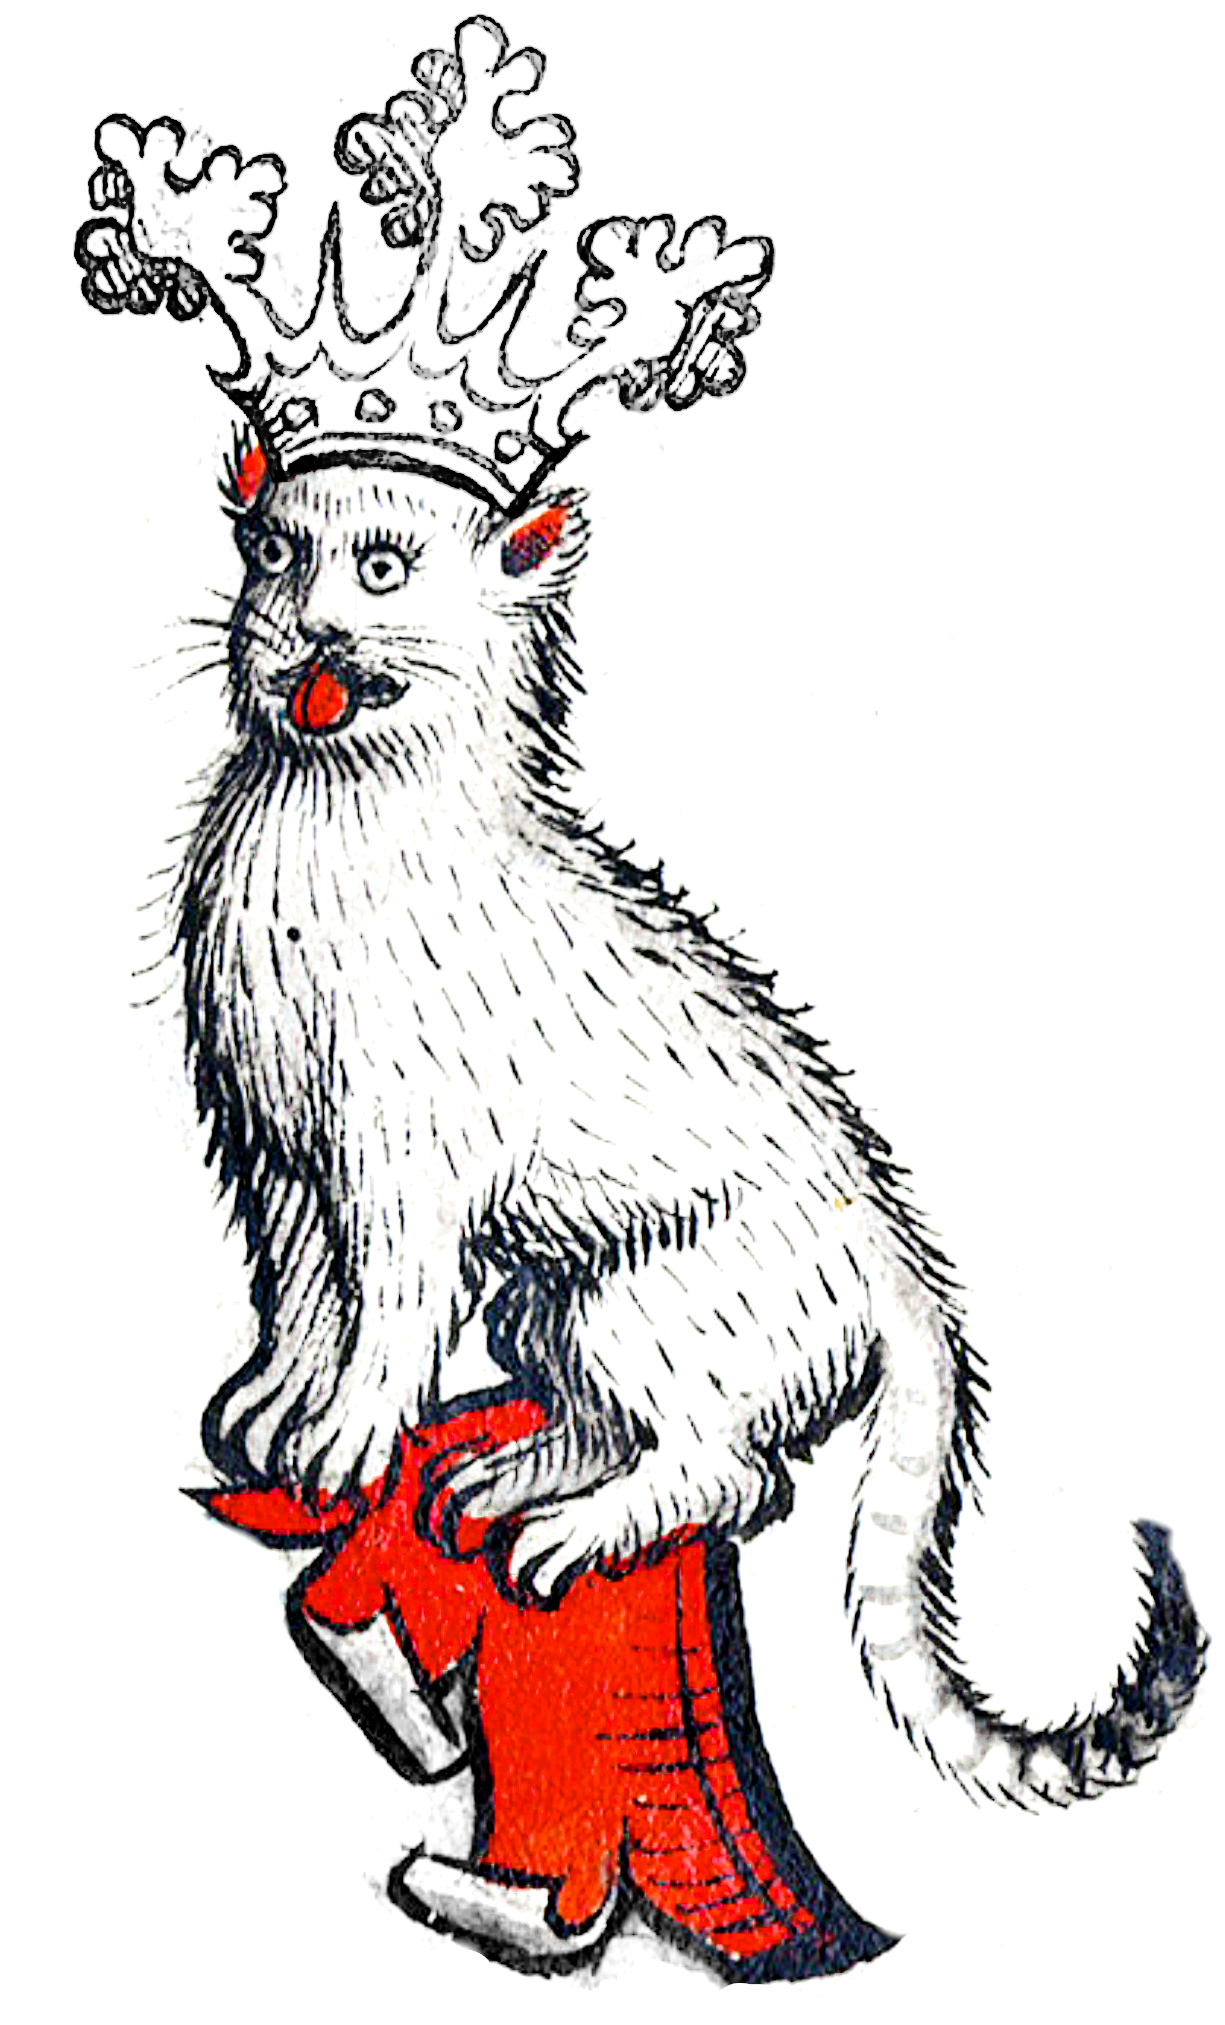
\includegraphics[width=6cm]{cat.png}
        % Cat sourced from:
        % https://www.reddit.com/r/MedievalCats/comments/e713ht/king_derpy/
        % Edited version on:
        % https://github.com/Kamik423/christmas-card-2019
        \vfill
        \begin{minipage}[c]{.8\columnwidth}
            \centering\large
            \c{``}Give a man a fire and he's warm for a day, but set fire to him
            and he's warm for the rest of his life.\c{''}\\[5mm]
            \c{--}Sir Terry Pratchett
        \end{minipage}
        \vfill
        \raisebox{1.5cm}[\height][0pt]{
            \pgfornament[anchor=north,width=1.5cm,symmetry=h]{63}
            \hspace{6cm}
            \pgfornament[anchor=north,width=1.5cm,symmetry=c]{63}
        }
        \vspace{9.5cm}~
    \end{multicols*}
\end{document}